\documentclass[12pt]{article}
\usepackage{geometry}
\usepackage[round]{natbib}
\geometry{margin=0.75in,textheight=7in}
 

\usepackage{amssymb}
\usepackage{amsmath}
\usepackage{amsfonts}
\usepackage{latexsym}
\usepackage[mathscr]{euscript}
\usepackage{mathrsfs}
\usepackage{graphicx}
\usepackage{comment}
\usepackage{cite}
\usepackage{multirow}
%\usepackage{mathtools} % \coloneqq and \eqqcolon
\usepackage{color}
\usepackage[table,xcdraw]{xcolor}
\usepackage{wrapfig}
\usepackage{amsmath}
\usepackage{tikz}
\usetikzlibrary{arrows}
\usetikzlibrary{external}
\tikzexternalize[prefix=tikz/]
% \tikzset{external/remake next} % Put this before figures to force remake 
\usepackage{pgfplots}
\usepackage{xspace}

\setlength{\textwidth}{6.5in}
\setlength{\oddsidemargin}{0.00in}      
\setlength{\topmargin}{-0.4in}
\setlength{\headheight}{0in}
\setlength{\textheight}{9.0in}  

\setlength{\parindent}{0em}
\setlength{\parskip}{1em}
%\renewcommand{\baselinestretch}{1.0}

\setlength{\belowdisplayshortskip}{0pt}
\setlength{\abovedisplayshortskip}{0pt}
\setlength{\abovedisplayskip}{0pt}
\setlength{\belowdisplayskip}{0pt}

\setlength{\parskip}{5pt}
\setlength{\parindent}{0in}

\title{Research Notes: Tabak-Rinzel, eupnea, sigh,\\  and calcium dynamics}
\author{Greg Conradi Smith, Daniel Scott Borrus, Christopher Del Negro }



\input{math_def}
\input{ca_def}


\def\pre{preB\"otC\xspace}
\def\ca{Ca$^{2+}$\xspace}

\def\w{w}
\def\taua{\tau_a}
\def\taus{\tau_s}
\def\thetaa{\theta_a}
\def\ka{k_a}
\def\thetas{\theta_s}
\def\ks{k_s}
\def\ainf{a_\infty}
\def\sinf{s_\infty}
\def\thetab{\theta_b}
\def\kb{k_b}
\def\thetac{\theta_c}
\def\kc{k_c}

\def\thetainf{\theta_\infty}
\def\tautheta{\tau_\theta}
\def\tauthetamax{\tau_\theta^{max}}
\def\tauthetamin{\tau_\theta^{min}}
\def\thetatheta{\theta_\theta}
\def\ktheta{k_\theta}
\def\thetatautheta{\theta_{\tautheta}}
\def\ktautheta{k_{\tautheta}}

\def\micromolar{\mu\mathrm{M}}
\def\uM{\micromolar}
\def\UM{$\uM$}
\def\persecond{\mathrm{s}^{-1}}
\def\permillisecond{\mathrm{ms}^{-1}}
\def\micromolarpersecond{\mu\mathrm{M}\,\mathrm{s}^{-1}}
\def\uMps{\micromolarpersecond}
\def\permicromolarpersecond{\mu\mathrm{M}^{-1}\,\mathrm{s}^{-1}}
\def\permolarpersecond{\mathrm{M}^{-1}\,\mathrm{s}^{-1}}
\def\puMps{\permolarpersecond}
\def\permicromolarpermillisecond{\mu\mathrm{M}^{-1}\,\mathrm{ms}^{-1}}
\def\puMpms{\permicromolarpermillisecond}

\def\xia{\xi_a}

\def\jin{j_{in}}
\def\jinzero{\jin^0}
\def\jinone{\jin^1}
\def\kout{k_{out}}
\def\ctot{c_{tot}}
\def\cer{c_{er}}
\def\rinf{r_\infty}
\def\minf{m_\infty}
\def\hinf{h_\infty}
\def\rinf{r_\infty}
\def\finf{f_\infty}
\def\thetam{\theta_m}
\def\thetar{\theta_r}
\def\km{k_m}
\def\thetah{\theta_h}
\def\kh{k_h}

\def\amax{a_{max}}
\def\smax{s_{max}}
\def\thetamax{\theta_{max}}

\begin{document}

\maketitle

\section*{An activity model of episodic bursting}

We model the eupnea subsystem in a manner similar to Tabak and Rinzel~\citeyearpar{TabakRinzel05}.  In the original Tabak-Rinzel model, the ODE representing network activity (firing rate) takes the form $\tau_a da/dt = \ainf (\w \cdot s \cdot d \cdot a) - a$ where $s$ and $d$ represent synaptic depression operating on a slow and fast time scales. 

The steady state activity is the following sigmoidal function of synaptic input ($x$): $\ainf(x) =  [1+e^{4(\thetaa-x)/\ka}]^{-1}$. 


Fast synaptic depression leads to oscillatory dynamics during the active phase of each burst.  These oscillations do not occur in our case, so 
the ODEs that are our starting point are
$\tau_a da/dt = \ainf (\w \cdot s \cdot a) - a$ and $
\taus ds/dt = \sinf (a) - s$ where the steady state activity (firing rate) is the following sigmoidal function of synaptic input ($x$): $\ainf(x) =  [1+e^{4(\thetaa-x)/\ka}]^{-1}$.  Similarly, the steady state synaptic depression is a sigmoidal function of network activity: $\sinf(a) =  [1+e^{4(\thetas-a)/\ks}]^{-1}$. Thus, our two state variables can be written 

\begin{eqnarray}
\tau_a \ddt{a} &=& \ainf (\w \cdot s \cdot a) - a\label{ODEa} \\
\taus \ddt{s} &=& \sinf (a) - s  \label{ODEs} 
\end{eqnarray}
where $a$ is the network activity and $s$ accounts for the dynamics of synaptic depression. Note that when $s=0$, the system is fully depressed.
The steady state functions $\ainf$ and $\sinf$ are given by 
\begin{eqnarray}
\ainf(x) &=& \frac{1}{1+e^{4(\thetaa-x)/\ka}}  \label{SQUASHA} \\
\sinf(x) &=& \frac{1}{1+e^{4(\thetas-x)/\ks}}  \label{SQUASHS} 
\end{eqnarray}
Note: When $\ka$ is positive (negative), $\ainf$ is a monotone decreasing (increasing) function of $x$, and similarly for $\ks$/$\sinf$.   The 4 that appears  in \EqsAnd{SQUASHA}{SQUASHS} makes $\ka$ and $\ks$ the inverse of the slope of $\ainf$ and $\sinf$ at the half-max.  

\Fig{AinfAndW} shows that depending on the strength (gain) of recurrent excitation, denoted by $\w$, the network activity can have 1--3 steady states. For intermediate values of $\w$ the excitatory network is  bistable.

The $a$ and $s$ nullclines are given by $a = \ainf(\w \cdot s \cdot a)$ and $s = \sinf(a)$.  The first expression is implicit, but it can be written explicitly by viewing $s$ as a function of $a$: 
\[
a~\mbox{nullcline:} \quad 
a = \ainf (\w \cdot s \cdot a )   \Longrightarrow s = \frac{4 \thetaa  - \ka \ln \left[ (1-a)/a \right] }{4 \w a} \, . 
\]

The system can be configured into two unique forms of excitability, depending on the parameters used. \Fig{HopfAndSNIC} shows nullclines with two parameter sets corresponding to type 2 (left) and type 1 (right) excitability. 

As we adapt this model to represent a population of firing neurons, it will be helpful to assign realistic units to the firing rate, $a$. Rather than $a$ representing the fraction of firing cells, we assign $a$ units of spikes per neuron per second. When this is the case, $a$ can be greater than 1, however the behavior of the $a$ nullcline doesn't change that much. When $\lim_{x \rightarrow \infty } \ainf(x)=\amax \neq 1$, the equation for the $a$ nullcline is
\[
a~\mbox{nullcline:} \quad 
a = \ainf (\w \cdot s \cdot a )   \Longrightarrow s = \frac{4 \thetaa  - \ka \ln \left[ (\amax-a)/a \right] }{4 \w a} \, . 
\]

\begin{figure}[h!]
\tikzset{every node/.style={font=\normalsize}}
\pgfplotsset{every axis/.style={
        clip=true,
        height=6cm,
        width=7cm,
        xmax=1.05,
        xmin=-0.05,
        ymin=-0.05,
        ymax=1.05,
        axis x line=bottom,
        legend pos=south east,
        xlabel={$a$},
        ylabel={$\ainf(\w a)$},
        axis y line=left,
        ylabel near ticks,
        xlabel near ticks,
        ylabel style={rotate=-90},
        domain=-0.1:1.1,
        samples=200]}}
\begin{center}
\begin{tikzpicture}
\def\figw{1}
\def\figthetaa{0.18}
\def\figka{0.2}
\begin{axis}[]
\addplot[blue,thick,dotted] {1/(1+exp(4*(\figthetaa-0.2*x)/\figka))}; 
\addlegendentry{$\w=0.2$}
\addplot[blue,thick] {1/(1+exp(4*(\figthetaa-0.4*x)/\figka))}; 
\addlegendentry{$\w=0.4$}
\addplot[blue,thick,dashed] {1/(1+exp(4*(\figthetaa-1.0*x)/\figka))}; 
\addlegendentry{$\w=1.0$}
\addplot[black] {x}; 
\end{axis}
\end{tikzpicture}
\end{center}
\caption{For intermediate values of $\w$ the excitatory network is bistable. Synaptic depression is off ($s=1$). Parameters: $\thetaa= 0.18$, $\ka=0.2$}
\label{AinfAndW}
\end{figure}


\begin{figure}
\tikzset{every node/.style={font=\normalsize}}
\pgfplotsset{every axis/.style={
        clip=true,
        height=6cm,
        width=7cm,
        xmax=1.05,
        xmin=-0.05,
        ymin=-0.05,
        ymax=1.05,
        axis x line=bottom,
        legend pos=north east,
        xlabel={$s$},
        ylabel={$a$},
        axis y line=left,
        ylabel near ticks,
        xlabel near ticks,
        ylabel style={rotate=-90},
        domain=0:1,
        samples=200]}}
\begin{tikzpicture}
\def\figw{1}
\def\figtaua{10}
\def\figthetaa{0.18}
\def\figka{0.2}
\def\figthetas{0.14}
\def\figks{-0.08}
\def\figthetassnic{0.42}
\def\figkssnic{-1.6}
\begin{axis}[]

\addplot[blue,thick] ({1/(1+exp(4*(\figthetas-x)/\figks))}, {x}); 
\addplot[red,thick,samples=400,domain=0:1,smooth]  ({(4*\figthetaa-\figka*ln(1/x-1))/(4*\figw*x)}, {x});

\draw[red,thick,dotted] (axis cs: 0.45,1) -- (axis cs: 1,1);
%\addplot[red,thick,samples=40,domain=0.99:1,smooth]  ({(4*\figthetaa-\figka*ln((1-x)/x))/(4*\figw*x)}, {x});
\end{axis}

\begin{axis}[xshift=7.0cm]

\addplot[red,thick,samples=400,domain=0:1]  ({(4*\figthetaa-\figka*ln(1/x-1))/(4*\figw*x)}, {x});
 \addlegendentry{$\dot{a}=0$}
 
\addplot[blue,thick] ({1/(1+exp(4*(\figthetassnic-x)/\figkssnic))}, {x});
\addlegendentry{$\dot{s}=0$}

\draw[red,thick,dotted] (axis cs: 0.45,1) -- (axis cs: 1,1);
%\addplot[red,thick,samples=40,domain=0.99:1]  ({(4*\figthetaa-\figka*ln((1-x)/x))/(4*\figw*x)}, {x});
\end{axis}

\end{tikzpicture}
\caption{Nullcines for the modified Tabak-Rinzel model.  Left: Type 2 oscillations; $\thetas=0.14$, $\ks=-0.08$.  Right: Type 1 excitability; $\thetas=0.42$, $\ks=-1.6$.  Other parameters: $\w=1$, $\taua=10$, $\thetaa= 0.18$, $\ka=0.2$.}
\label{HopfAndSNIC}
\end{figure}



% Figure showing several possible nulc lines for a depending on thetaa
% I'm removing, since it isn't as useful once the third state variable is introduced
% DB 12/9/2020

% \begin{figure}
% \centering 
% \tikzset{every node/.style={font=\normalsize}}
% \pgfplotsset{every axis/.style={
%         clip=true,
%         height=6cm,
%         width=7cm,
%         xmax=1.05,
%         xmin=-0.05,
%         ymin=-0.05,
%         ymax=1.05,
%         axis x line=bottom,
%         legend pos=north east,
%         legend style={font=\footnotesize,legend cell align=right},
%         xlabel={$s$},
%         ylabel={$a$},
%         axis y line=left,
%         ylabel near ticks,
%         xlabel near ticks,
%         ylabel style={rotate=-90},
%         domain=0:1,
%         samples=200]}}
% \begin{tikzpicture}
% \def\figw{1}
% \def\figtaua{10}
% \def\figthetaa{0.18}
% \def\figka{0.2}
% \def\figthetas{0.14}
% \def\figks{-0.08}
% \def\figthetassnic{0.42}
% \def\figkssnic{-1.6}
% \begin{axis}[restrict x to domain=0:1,thick]


% \addplot[red,dotted] ({(4*0.09-\figka*ln(1/x-1))/(4*\figw*x)}, {x});
% \addlegendentry{$\thetaa=0.09$}

% \addplot[red,dashdotted] ({(4*0.14-\figka*ln(1/x-1))/(4*\figw*x)}, {x});
% \addlegendentry{$0.14$}

% \addplot[red,dashed]  ({(4*0.18-\figka*ln(1/x-1))/(4*\figw*x)}, {x});
% \addlegendentry{$0.18$}

% \addplot[red]  ({(4*0.19-\figka*ln(1/x-1))/(4*\figw*x)}, {x});
% \addlegendentry{$0.19$}

% \addplot[blue,thick] ({1/(1+exp(4*(\figthetas-x)/\figks))}, {x}); 
% \end{axis}

% \end{tikzpicture}
% \caption{Nullcines for the modified Tabak-Rinzel model using a range of values for $\thetaa$ (standard value is $0.18$). Other parameters: $\w=1$, $\ka=0.2$.
% }
% \label{HopfStudy}
% \end{figure}


\clearpage
\subsection*{Noise}


So far we have assumed deterministic dynamics.  Intrinsic stochastic dynamics of the excitatory network is modeled by additive Gaussian white noise with state-dependent variance to \Eq{ODEa}. The model is now written
\begin{eqnarray}
\tau_a \ddt{a} &=& \ainf (\w \cdot s \cdot a) - a + \hat{\xia}(a(t)) \label{ODEAnoise} \\
\taus \ddt{s} &=& \sinf (a) - s  \label{ODESnoise} 
\end{eqnarray}
The noise term has mean zero, i.e., $\langle \hat{\xia} \rangle = 0$.  The variance of the Gaussian white noise is derived by considering the rates of the forward and reverse  elementary processes
implied by the deterministic ODE for the network activity. Consider the deterministic part of \Eq{ODEa}:
\begin{equation*}
 \ddt{a} = \dfrac{ \ainf(wa) - a }{\taua} 
\end{equation*}
where we 
note that $\lim_{x \rightarrow -\infty} \ainf(x)=0$ and
write $\amax$ for the limit of $\ainf(x)$ as $x \rightarrow \infty$.  Defining 
\begin{equation*}
\taua = \frac{1}{\alpha+\beta } \quad \mbox{and} \quad \ainf = \dfrac{\alpha}{\alpha+\beta} \amax  
\end{equation*}
we have 
\begin{equation*}
\alpha  = \frac{\ainf}{\amax \taua } \quad \mbox{and} \quad \beta = \dfrac{\amax - \ainf}{\amax \taua}   
\end{equation*}
Thus \Eq{ODEa} can be written as 
\begin{equation*}
 \ddt{a} = \alpha (\amax - a) - \beta a  
\end{equation*}
This is consistent with the elementary processes shown in this diagram:
\begin{center}
\begin{tikzpicture}
\draw[] (0,0) node[draw,rounded corners,minimum size=1cm] (aleft) {$a_{max}-a$};
\draw[] (3,0) node[draw,rounded corners,minimum size=1cm] (aright) {$a$};
\draw[bend left,-latex,thick] (aleft) to node[above] (forward) {$\alpha = \dfrac{\ainf}{\amax\taua}$} (aright);
\draw[bend left,-latex,thick] (aright) to node[below] (reverse) {$\beta = \dfrac{ \amax-\ainf}{\amax\taua}$} (aleft);
\end{tikzpicture}
\end{center}
This leads to the following expression for the two-time covariance 
\[
\langle \hat{\xia} (t) \hat{\xia} (t')  \rangle = \gamma_a (a,s) \delta (t - t')
\]
where 
\begin{equation}
  \gamma_a (a,s) = \frac{1}{N} \left[  \alpha \cdot (\amax-a) + \beta \cdot a \right] = 
  \frac{1}{N \amax \taua } \left[  \ainf \cdot (\amax-a) + (\amax - \ainf)  a \right] \label{SizeOfFluctuations}
\end{equation}
Figure \ref{SizeOfFluctuationsgraph} describes the size of the fluctuations as a function of the activity level.


\begin{figure}[t!]
\tikzset{every node/.style={font=\normalsize}}
\pgfplotsset{every axis/.style={
        clip=true,
        height=6cm,
        width=8cm,
        xmax=1.05,
        xmin=-0.05,
        ymin=-0.05,
        ymax=1.25,
        axis x line=bottom,
        legend pos=north west,
        xlabel={$a$},
        ylabel={$\left[  \ainf \cdot (\amax-a) + (\amax - \ainf)  a \right]$},
        axis y line=left,
        ylabel near ticks,
        xlabel near ticks,
        ylabel style={rotate=-90},
        domain=-0.1:1.1,
        samples=200]}}
\begin{center}
\begin{tikzpicture}

\def\figw{1}
\def\figthetaa{0.18}
\def\figka{0.2}
\def\figN{100}
\def\figamax{1}
\def\figtaua{1}
\begin{axis}[]
 
% \addplot[blue, ultra thin] {(1/(1+exp(4*(\figthetaa-0.1*x)/\figka)))*(\figamax-x)+(\figamax-(1/(1+exp(4*(\figthetaa-0.1*x)/\figka))))*x};
% \addlegendentry{$s=0.1$}

\addplot[blue, dashed] {(1/(1+exp(4*(\figthetaa-0.2*x)/\figka)))*(\figamax-x)+(\figamax-(1/(1+exp(4*(\figthetaa-0.2*x)/\figka))))*x};
\addlegendentry{$s=0.2$}

\addplot[blue, dotted, thick] {(1/(1+exp(4*(\figthetaa-0.5*x)/\figka)))*(\figamax-x)+(\figamax-(1/(1+exp(4*(\figthetaa-0.5*x)/\figka))))*x};
\addlegendentry{$s=0.5$}

\addplot[blue] {(1/(1+exp(4*(\figthetaa-0.9*x)/\figka)))*(\figamax-x)+(\figamax-(1/(1+exp(4*(\figthetaa-0.9*x)/\figka))))*x};
\addlegendentry{$s=0.9$}

% \addplot[blue,thick,solid] {1/(1+exp(4*(\figthetaa-0.9*x)/\figka)) + x - 2*x/(1+exp(4*(\figthetaa-0.9*x)/\figka))}; 
%\addlegendentry{$s=0.9$}
 
\end{axis}
\end{tikzpicture}
\end{center}
\caption{Size of fluctuations as given by Eq. \ref{SizeOfFluctuations}. The size of the noise depends on the network firing rate $a$ and synaptic depression $s$. Other parameters are the default values: $\theta_a=0.18$, $k_a=0.2$, $w=1$.}
\label{SizeOfFluctuationsgraph}
\end{figure}


\clearpage
\subsection*{System limitations arising from one slow variable}

Our current system has one fast variable, $a$ the network firing rate, and one slow variable, $s$ the average synaptic depression in the network. With this fast-slow system we are able to generate network oscillations. Figure \ref{TabakRinzelOneVarIntro}B depicts the trajectories of $a$ and $s$ when the system is configured for type 2 excitability. Here, the oscillations arise from a supercritical-hopf bifurcation (HB), and the appearance of a stable limit cycle. (should we include the bif. diagram?)

How well does this configuration of the model match with what we see in the preB\"otC experimentally? 


The timing between each burst event is normally distributed, just like it is in the biology. The events are normal distributed because membrane noise either increases or decreases the total time synaptic depression can recover. However, this will lead to a problem with burst size.

We can see the noise manifest in the system at the bottom knee of the $a$ nullcline. Now, each burst has a slight variation in the magnitude of its synaptic depression. This proves to be critical to the behavior of the system. If a burst is delayed, then the synaptic depression term recovers to a greater degree, and the ensuing burst will be larger. Ultimately, this leads to a phenomenon whereby bursts with longer preceding intervals have a larger burst area. There is a correlation between preceding interval and burst size. This has consequences for bursts that are initiated prematurely. Bursts that are ``kicked'' into the limit cycle early will ultimately terminate early, because synaptic depression hasn't fully recovered, and so ends the burst early. This is not observed experimentally. 

First, there is no relationship between the preceding interval and the burst amplitude or area experimentally. (NEED FIGURE). Second, as was shown by CDN 2009 (FIX), there is a refractory period after a \pre burst during which another network burst cannot be elicited. After that refractory period has expired, a burst can be evoked but the amplitude and area are not dependent on the time since the previous burst or the end of the refractory period. In the type-2 excitability configuration, burst events in the model will always depend on the magnitude of synaptic depression recovery. This problem can be resolved when we shift the model into type-1 excitability.  

Figure \ref{TabakRinzelOneVarIntro}B depicts the system in type-1 excitability. Here the system is subcritical to a saddle-node on an invariant circle (SNIC) bifurcation. Now the synaptic depression recovers to a maximum value before every burst. The burst size is no longer dependent on the duration of the preceding inter-event interval. Because the system is subcritical, it will not fire without some sort of noise. Membrane noise drives the system over the threshold, and triggers an event. Herein lies another problem.

The membrane noise is driven by a Wiener process, or brownian motion. As we wait for the noise to integrate above some threshold, we are waiting for a random event with some known probability to occur. This is Poisson process, and the timing between successive events will follow an exponential distribution. Indeed, in our model in a type-1 configuration, the timing between burst events appears to be exponentially distributed (after some minimal time). We know breaths are not exponentially distributed \textit{in vivo}. That would be a terrifying phenomenon. We can also show burst events are not exponentially distributed in the \pre \textit{in vitro}. (FIGURE)

Thus we are at an impasse with our two variable model. In the type-2 configuration, the timing between the events is normally distributed, but there is an undesirable relationship between the size of the burst events and the duration of the preceding interval. In the type-1 configuration, similar to the biology, there is no relationship between burst size and the preceding interval. However, here the timing between the events is exponentially distributed, which does not represent the biology. From here, in order to bring our model into agreement with what we observe physiologically, we reasoned we needed an additional slow variable. 

\begin{figure}[h!]
\centering 
 \includegraphics[width=\textwidth]{Fig01TabakRinzelOneVarIntro}
\caption{Draft figure for our argument that the eupnea model requires two slow variables. }
\label{TabakRinzelOneVarIntro}
\end{figure}


\clearpage
\section*{The eupnea model}

We model the eupnea subsystem using the following modifications of the Tabak-Rinzel-like model presented in the previous section. However, 
we include both synaptic depression ($s$) and 
cellular adaptation ($\theta$). 
The ODEs for our modification of the Tabak-Rinzel model are
\begin{eqnarray}
\tau_a \ddt{a} &=& \ainf (\w \cdot s \cdot a - \theta) - a + \hat{\xia}(a(t)) \label{ODEA} \\
\taus \ddt{s} &=& \sinf (a) - s  \label{ODES} \\
\tautheta(a) \ddt{\theta} &=& \thetainf (a) - \theta   \label{ODETHETA} 
\end{eqnarray}
where the variable  $\theta$ is an adaptive threshold for the activity as a function of synaptic input. 
The steady state functions $\ainf$ and $\sinf$ are given by \EqsAnd{SQUASHA}{SQUASHS}.  The steady-state function $\thetainf$ is analogous:
\begin{equation}
\thetainf(x) = \frac{1}{1+e^{4(\thetatheta-x)/\ktheta}} \label{SQUASHTHETA} \, . 
\end{equation}

The logic behind including cellular adaptation is described in the section above. In brief, recovery of synaptic depression happens long before the end of the silent phase, therefore there must be a second low variable.
The dependence of $\tautheta$ on the activity level is chosen to be 
\begin{equation}
    \tautheta(x) = \frac{\tauthetamax - \tauthetamin}{1+e^{4(\thetatautheta-x)/\ktautheta}}  + \tauthetamin \, . 
\end{equation}
This is important because the cellular adaptation needs to happen quickly in the active phase (when $a$ is large), but recover slowly during the silent phase (when $a$ is small). Figure \ref{TabakRinzelTwoVarRepresentative} demonstrates the three state system undergoing oscillations. Synaptic depression terminates the bursts, and the recovery of the adaptation variable ($\theta$) determines the timing of the subsequent burst. 

The mathematical model for eupnea generation is inline with what we observe biologically. The timing between the events in normally distributed. And there is no relationship between the preceding interval and the size of the subsequent burst. (ADD TWO MORE FIGURES HERE DB).

Table \ref{ParamDefEupnea} describes the default parameters used for the eupnea subsystem. 

\begin{figure}
\centering 
\includegraphics[width=\textwidth]{Fig02TabakRinzelTwoVarRepresentative}
\caption{Draft figure showing Tabak-Rinzel like model with two slow variables ($s$ and $\theta$). }
\label{TabakRinzelTwoVarRepresentative}
\end{figure}

\begin{table}[h!]
\centering 
\begin{tabular}{clcc}
    Symbol & Definition & Value  & Units \\
\hline 
\hline
$w$ & network connectivity & 1 &  - \\
\hline 
\hline 
$\theta_a$ & average firing threshold  (half activation) &  $[-0.3,0.1]$ & \\
$k_a$ & reciprocal of slope of $\ainf$ at half activation  & 0.2 &  \\
$\tau_a$ & network recruitment time constant  & 0.15  & \\
\hline 
$\theta_s$ & half activation of $s$ & 0.14 &  \\
$k_s$ & reciprocal of slope of $\sinf$ at half activation  & -0.08 &  \\
$\tau_s$ & time constant of synaptic depression   & 0.75 &  \\
\hline 
$\thetatheta$ & half activation of $\theta$ & 0.15 &  \\
$k_\theta$ & reciprocal of slope of $\thetainf$ at half activation  & 0.2 &  \\
\hline 
$\tauthetamax$ & maximum of time constant of cellular adaptation   & 6 &  \\
$\tauthetamin$ &  minimum of time constant of cellular adaptation   & 0.15 & \\
$\thetatautheta$ & half max of $\tautheta(a)$  & 0.3 &  \\
$\ktautheta$ & reciprocal of slope of $\tautheta(a)$ at half activation  & -0.5&   \\
    \hline 
    \hline
\end{tabular}
\caption{Description of parameters for eupnea model and standard values.}
\label{ParamDefEupnea}
\end{table}

\clearpage          
\section*{The sigh model: calcium handling}

\subsection*{Closed cell Ca$^{2+}$ model with bistability}

We propose the sigh rhythm emerges from intracellular Ca$^{2+}$ dynamics. We borrow the template for modeling \ca handling from Keizer and Levine 1996. Our description of the equations begins with a closed system, where the total calcium in the cell is fixed and calcium moves between the cytosol and intracellular \ca stores, such as the ER.

\begin{eqnarray}
  \ddt{c} &=&  \left[ v_1  \rinf (c)+ v_2 \right] (\cer - c ) - \frac{v_3 c^2}{k_3^2+c^2} \label{closedcac1}\\
  \cer &=& (\ctot-c)/\lambda \label{closedcac2}
\end{eqnarray}

$v_1r_\infty(c)$ describes \ca leaving the ER via \ca-induced-\ca-release. $v_2$ describes passive \ca leak from the ER to the cytosol. $v_3$ controls the rate of \ca in the cytosol being pumped into the ER via SERCA pumps on the walls of the ER. The phase diagram for Eq. \ref{closedcac} is shown in Figure \ref{CalciumClosedCell}. Depending on the total calcium in the cell, there are 1--3 steady states for the \ca subsystem.

\def\figthetam{0.25}
\def\figkm{0.04}
\def\figthetah{0.3}
\def\figkh{-0.06}
\def\figlambda{0.15}
%\def\figctot{1}
\def\figvone{40}
\def\figvtwo{0.5}
\def\figvthree{120}
\def\figkthree{0.3}


\begin{figure}[h!]
\centering
%\includegraphics[]{Fig10CaDynamics.pdf}
\includegraphics[]{Fig03CalciumClosedCellModel.pdf}
\caption{Closed cell model. Parameters: 
$\thetam=\figthetam$,
$\km=\figkm$,
$\thetah=\figthetah$,
$\kh=\figkh$,
$\lambda=\figlambda$,
$v_1 = \figvone$,
$v_2 = \figvtwo$,
$v_3 = \figvthree$, 
$k_3 = \figkthree$.
}
\label{CalciumClosedCell}
\end{figure}
 
\clearpage
\subsection*{Open cell Ca$^{2+}$ model} 

Eqs. \ref{closedcac1} and \ref{closedcac2} can be modified to allow for \ca fluxes across the plasma membrane. The \ca concentration in the cell is no longer fixed. $\jmath_0$ controls the \ca flux into the cytosol from outside the cell. $v_4$ regulates the rate \ca is pumped out of the cell. The concentration of \ca in the ER can be determined at any time by subtracting the total \ca concentration by the \ca concentration in the cytosol. $\lambda$ accounts for the change in volume between the cytosol and ER. 

\begin{eqnarray*}
  \ddt{c} &=&  \left[ v_1 \finf(c) + v_2 \right] [\cer - c ] - \frac{v_3 c^2 }{\kappa_3^2 + c^2} + \jmath_0    -  \frac{v_4 c^4}{\kappa_4^4+c^4} \\
 \ddt{\ctot} &=& \jmath_0  -   \frac{v_4 c^4}{\kappa_4^4+c^4}
\end{eqnarray*}
where  $\cer = (\ctot-c)/\lambda$ and 
\begin{equation}
\finf(c) =  \frac{1}{1+e^{(\thetam-c)/\km}} \cdot  \frac{1}{1+e^{(\thetah-c)/\kh}}  \nonumber 
\end{equation}
where $\km>0$ and $\kh<0$. $f_\inty(c)$ still describes the rate of \ca-induced-\ca-release and takes the form of a bell shaped curve. The dynamics of the open cell \ca subsystem are described in Figure \ref{opencamodel}. Default parameters are written in Table \ref{ParamDefCalcium}.

\begin{figure}[h!]
    \centering
    \includegraphics{Fig03CalciumOpenCellModel.pdf}
    \caption{Open cell calcium dynamics. Calcium subsystem only.}
    \label{opencamodel}
\end{figure}

\begin{table}[h!]
\centering 
\begin{tabular}{clcc}
    Symbol & Definition & Value &Units  \\
\hline 
\hline
$v_1$ & rate constant of calcium release & 20  & $\persecond$  \\
$v_2$ & rate constant of calcium leak   & 0.25 & $\persecond$ \\
$v_3$ & maximum rate of SERCA pumps & 60  &  $\micromolarpersecond$  \\
$k_3$ & half maximum for SERCA pumps  & 0.3 & $\micromolar$ \\
$n_3$ & Hill coefficient for SERCA pumps   & 2 & - \\
$\lambda$ & ER/cytosol effective volume ratio & 0.15 & - \\
$\thetam$ & activation of intracellular calcium channels & 0.25 & $\micromolar$ \\
$\km$ & reciprocal of slope of   $\minf$ at half maximum & 0.04 & - \\
$\thetah$ & activation of intracellular calcium channels & 0.3 & $\micromolar$\\
$\kh$ & reciprocal of slope of   $\hinf$ at half maximum & -0.06 & - \\
    \hline 
 $\jinzero$ & constant calcium influx rate  & 0.009 & $\micromolarpersecond$ \\
  $\jinone$ &  calcium influx rate  proportionality constant & 0.02 & $\micromolarpersecond/activity$ \\
  $v_4$ & maximum rate of PMCA pumps & 0.4  & $\micromolarpersecond$ \\
$k_4$ & half maximum for PMCA pumps  & 0.3 & $\micromolar$ \\
$n_4$ & Hill coefficient for PMCA pumps   & 4 & - \\

    \hline
\end{tabular}
\caption{Description of parameters for calcium handling and standard values.}
\label{ParamDefCalcium}
\end{table}

\clearpage
\section*{The Tabak-Rinzel-like activity model with calcium dynamics}

We connected the eupnea and calcium subsystems to model the two simultaneous rhythms in \pre, inspiratory and sigh breaths. 

\begin{eqnarray*}
\tau_a \ddt{a} &=& \ainf (\w \cdot s \cdot a -\theta , c) - a + \hat{\xi}(a) \label{ODEACALCIUM} \\
\taus \ddt{s} &=& \sinf (a) - s  \label{ODESCALCIUM} \\
\tautheta(a) \ddt{\theta} &=& \thetainf (a) - \theta   \label{ODETHETACALCIUM}  \\
  \ddt{c} &=&  \left[ v_1 \finf(c) + v_2 \right] [\cer - c ] - \frac{v_3 c^2 }{\kappa_3^2 + c^2} + \jmath_0 + \jmath_1 a   -  \frac{v_4 c^4}{\kappa_4^4+c^4}  \label{ODESCALCIUM} \\
 \ddt{\ctot} &=& \jmath_0 + \jmath_1 a -   \frac{v_4 c^4}{\kappa_4^4+c^4}   \label{ODESCALCIUM}  \label{ODESCAER}
\end{eqnarray*}
where  $\cer = (\ctot-c)/\lambda$ and 
\begin{equation}
\finf(c) =  \frac{1}{1+e^{(\thetam-c)/\km}} \cdot  \frac{1}{1+e^{(\thetah-c)/\kh}}  \nonumber 
\end{equation}
where $\km>0$ and $\kh<0$.  We assume that the 
steady state function $\ainf$ is `boosted' by the intracellular calcium concentration, as follows:
\begin{equation}
\ainf(x,c) = \frac{\lambda_a }{1+e^{4(\thetaa-x)/\ka}}  + \frac{\lambda_c }{1+e^{4(\thetac-c)/\kc}}  
 \nonumber 
\end{equation}
% %where $\lambda_c=1-\lambda_a$ and $0 \leq \lambda_a \leq 1$ and similarly for $\lambda_c$.
% (In preliminary modeling, I used
% \begin{equation}
% \ainf(x,c) = \frac{ 1 }{1+e^{4(\thetaa-x)/\ka}} \left( 1 +  \frac{v_5 c^4}{\kappa_5^4+c^4} \right) 
%  \nonumber \, .
% \end{equation}
% This did not work well, because the boosting could be vetoed by synaptic depression and cellular adaptation.)
where $\lambda_c$ is the contribution of intracellular \ca to network activity. This is comparable to activation of a \ca-activted Na$^+$ current (I$_{\text{CAN}}$). Activity is tied back into the \ca subsystem via the $\jmath_1$ term. When activity is high, \ca enters the cytosol at a rate proportional to $\jmath_1$. These terms are responsible for welding the two subsystems together. 


The steady state cytosolic calcium concentration solves the implicit expression 
\begin{equation*}
0= (v_1 + v_2 \rinf (c) ) \left(\frac{\ctot-c}{\lambda} - c \right) - \frac{v_3 c^2 }{\kappa^2 + c^2} + \jmath_0 + \jmath_1 a -   \frac{v_4 c^4}{\kappa_4^4+c^4}  \, , 
\end{equation*}
but this can be written as an explicit expression for $\ctot$ as a function of $c$,
\begin{equation*}
\ctot = (\lambda+1 )  c  -  \frac{\lambda }{ v_1 + v_2 \rinf (c) } \left( - \frac{v_3 c^2 }{\kappa^2 + c^2} + \jmath_0 + \jmath_1 a -   \frac{v_4 c^4}{\kappa_4^4+c^4} \right) 
\end{equation*}.
The steady state total calcium concentration can also be calculated.
\begin{align*}
    0 &= \jmath_0 + \jmath_1 a -   \frac{v_4 c^4}{\kappa_4^4+c^4} \\
    c &= \Big(\frac{\kappa_4^4(\jmath_0 + \jmath_1 a)}{v_4-\jmath_0 + \jmath_1 a}\Big)^{1/4}
\end{align*}

Trajectories of the entire system are shown in Figure \ref{EupneaAndSighRepresentative}. The faster eupnea oscillation and the slower sigh oscillation run in parallel.

\begin{figure}[h!]
\centering
\includegraphics[width=\textwidth]{Fig04EupneaAndSighRepresentative.pdf}
\caption{Draft figure of open cell model showing eupnea and sigh.}
\label{EupneaAndSighRepresentative}
\end{figure}

\clearpage
\section*{Eupnea and Sigh Voltage Dependence - Testable prediction \#1}


\begin{figure}[h!]
\centering
\includegraphics[width=\textwidth]{Fig05EupneaAndSighFrequency}
\caption{How excitability influences   eupnea and sigh frequency.   }
\label{EupneaAndSighFrequency}
\end{figure}

\section*{Bombesin-like peptide modulating sigh frequency -- Testable predicition \#2}

\section*{Calcium influx and coupling strength vs. eupnea/sigh timings -- Testable prediction \#3}

\section*{High j0 should lead to faster Ca oscillations, and sighs -- Testable prediction \#4}

Problem with this is, $\Delta$ Ca will influence eupnea frequency, which has a small, but non zero effect on sigh frequency.

\section*{Larger bursts will lead to high Ca influx during each eupniec burst, increasing sigh freq and increasing coupling-- Testable prediction \#5}

\section*{block Glia (purinergic?) signaling}

\section*{visualizing ER Ca fluxes with fluorescent indicators}

\nocite{TabakEtal00,TabakEtal01,TabakRinzel05}

\bibliographystyle{plainnat}
\bibliography{eupnea_sigh}

\newpage

\section*{SCRAPS}


\subsection*{Jacobian of Tabak-Rinzel-like model}

If $\taus$ is a constant, then 
the Jacobian of \EqsAnd{ODEA}{ODES} is 
\begin{equation*}
    J (a,s) = \begin{pmatrix}
     \left[ ws\ainf'(wsa)-1\right]/\taua  &     wa\ainf'(wsa) /\taua \\
     \sinf'(a)/\taus & -1/\taus \\
    \end{pmatrix}
\end{equation*}
where 
the steady state functions $\ainf$ and $\sinf$ are given by 
\begin{eqnarray}
\ainf'(\theta) &=& -4\frac{e^{4(\thetaa-\theta)/\ka}/\ka}{\left( 1+e^{4(\thetaa-\theta)/\ka} \right)^2 }  \nonumber \\
\sinf'(\theta) &=& -4\frac{e^{4(\thetas-\theta)/\ks}/\ks}{\left( 1+e^{4(\thetas-\theta)/\ks} \right)^2 }  \nonumber \\ \nonumber 
\end{eqnarray}
The condition for stability is $\mbox{tr}\, J < 0$ and $\mbox{det}\,J>0$.


\subsection*{\boldmath $\ainf$ with three inflection points}

\def\figw{0.4}
\def\figthetaa{0.1}
\def\figka{0.1}
\def\figthetab{0.3}
\def\figkb{0.1}
\def\figlambda{0.5}

\begin{figure}[h!]
\tikzset{every node/.style={font=\Large}}
\pgfplotsset{every axis/.style={
        clip=true,
        height=8cm,
        width=9cm,
        xmax=1.05,
        xmin=-0.05,
        ymin=-0.05,
        ymax=1.05,
        axis x line=bottom,
        legend pos=south east,
        xlabel={$a$},
        ylabel={$\ainf(\w a)$},
        axis y line=left,
        ylabel near ticks,
        xlabel near ticks,
        ylabel style={rotate=-90},
        domain=-0.1:1.1,
        samples=200]}}
\begin{center}
\begin{tikzpicture}


\begin{axis}[]
\addplot[black] {x}; 

\addplot[red,thick] {1/(1+exp(4*(\figthetaa-\figw*x)/\figka)) }; 
\addplot[green,thick] { 1/(1+exp(4*(\figthetab-\figw*x)/\figkb)) }; 
\addplot[blue,thick] {(1-\figlambda)/(1+exp(4*(\figthetaa-\figw*x)/\figka))
+ \figlambda/(1+exp(4*(\figthetab-\figw*x)/\figkb))
}; 
\addlegendentry{$\w=\figw$}

\end{axis}
\end{tikzpicture}
\end{center}
\caption{Parameters: $\w=\figw$, 
$\thetaa=\figthetaa$, 
$\ka=\figka$,
$\thetab=\figthetab$, 
$\kb=\figkb$, $\lambda=\figlambda$.}
\label{AinfAndWTwo}
\end{figure}

\begin{equation*}
 \ainf(x) = \frac{1-\lambda}{1+e^{4(\thetaa-x)/\ka}}    + \frac{\lambda}{1+e^{4(\thetab-x)/\kb}} 
\end{equation*}
 
 
%  \begin{equation}
%  =  
%   \frac{1}{N \amax \taua } \left[  \ainf \amax - \ainf a + \amax a - \ainf a \right]
%   =  
%   \frac{1}{N \amax \taua } \left[  \ainf \amax - (\amax - 2 \ainf) a  \right]\label{SizeOfFluctuations}
% \end{equation}
% where we have used $\ainf\cdot (1-a) + (1-\ainf) \cdot a = \ainf - \ainf a + a - \ainf a = \ainf - 2\ainf a+ a =  \ainf +  (1- 2\ainf) a$.
 
%\newpage
\subsection*{Constraining the new noise term - 4/23/20}
What is the correct amount of noise for our model? Currently, the only noise in the model is network activity fluctuations driven by a stochastic process in the activity ODE $a$. The equation for the $a$ ODE is written (in the code):
\[\dot{a} = \frac{a_\infty - a}{\tau_a} + \texttt{randn} \cdot \texttt{dt} \sqrt{1/\texttt{dt}/N/\tau_a/\amax \cdot\left[  \ainf \cdot (\amax-a) + (\amax - \ainf)  a \right]}
\]

As $N$ is our dial for the amount of noise in the system, the question is, what is an appropriate $N$ for our system? One idea to set this parameter is to compare the duration of inter-event-intervals we observe in the biology. Then to match increase noise in our simulation until we have a similar distribution of inter-event-durations.

I used 7 field recordings experiments and calculated the mean, sd, and coefficient of variation (cv) of the burst intervals. All intervals excluded sigh events.


\begin{table}[h!]
\center
\begin{tabular}{|l|l|l|l|}
\hline
Date    & $\mu$ & $\sigma$ & c.v. \\ \hline
180215  & 6.0 s& 1.9 s   & 0.32 \\ \hline
180309  & 7.0 s& 1.3 s   & 0.19 \\ \hline
080322  & 5.7 s& 0.9 s   & 0.16 \\ \hline
180420  & 7.6 s& 1.4 s   & 0.18 \\ \hline
180430  & 7.7 s& 2.8 s   & 0.36 \\ \hline
180515  & 5.6 s& 0.8 s   & 0.14 \\ \hline
180518  & 3.4 s& 0.7 s   & 0.22 \\ \hline
\rowcolor[HTML]{9AFF99} 
Average & 6.1 s& 1.1 s    & 0.23 s \\ \hline
\end{tabular}
\end{table}

Note, if we calculate cv on the averages, it's closer to cv = 0.19. Now that we have a desired distribution of inter-event-intervals, we can see how close we can get our simulation to the real data. Figure \ref{ChangingNoise} shows what happens when we modulate noise in the model, and how close we can get to the actual recordings. Table \ref{ChangingNoiseTable} holds the key statistics of this test.

\begin{table}[h!]
\center
\begin{tabular}{|l|l|l|l|l|l|l|l|}
\hline
$n$      & $\infty$ & 1000 & 100  & 50   & 20   & 1    & $10^*$ \\ \hline
$\sigma$ & 0        & 0    & 0.1  & 0.1  & 0.2  & 1.2  & 0.5    \\ \hline
$\mu$    & 4.3      & 4.3  & 4.3  & 4.3  & 4.3  & 3.8  & 4.3    \\ \hline
c.v.     & 0        & 0.01 & 0.02 & 0.03 & 0.04 & 0.31 & 0.11   \\ \hline
\end{tabular}
\caption{For last column *: $\lambda_a$ decreased from 20 to 7 spikes/neuron/second}
\label{ChangingNoiseTable}
\end{table}

\begin{figure}[h!]
\includegraphics[scale=0.6]{NoiseNotes/0_RealDataSet.png}
\includegraphics[scale=0.6]{NoiseNotes/3_100neurons.png} \\
\includegraphics[scale=0.6]{NoiseNotes/4_20neurons.png}
\includegraphics[scale=0.6]{NoiseNotes/5_10neuronsANDlowlambdaa.png}
\caption{Top left: Simulated distribution from the physiological parameters. Notice the wide distribution in spike interval durations. Top right: In red, a trace of the simulated activity. Below in blue, the histogram showin interevent durations in seconds. Top right plot has the low noise, where $N=100$. Bottom left has higher noise, but not high enough to have similar timing variability to physiological data. To get highest possible noise in physiological ranges, bottom right shows $N=10$ and $\lambda_a=7$. This gets a c.v. of only half the physiological norm.}
\label{ChangingNoise}
\end{figure}

We find that as N decreases, and the noise gets larger, our cv for event intervals doesn't get very large. Once we have 20 neurons in the simulation, the variability in event timing is still too small. We don't see large variability in eupnea timing in the model like we see in physiological data. Question for Greg \& me to think about, 

\begin{itemize}
    \item is it cheating to move $N$ extremely low? Like $<1$?
    Probably.
    \item Maybe a better idea is to introduce a second type of noise to the model... I know we discussed $\ca$ noise, but that won't help with this discrepancy between observed data and simulated results.
\end{itemize} 

\subsection*{s nulcline}

\begin{align*}
    \taus \frac{ds}{dt} &= \sinf(a)-s \\
    0 &= \frac{1}{1+e^{4(\thetas-a)/\ks}} - s_{ss} \\
    s_{ss} &= \frac{1}{1+e^{4(\thetas-a)/\ks}}\\
    1+e^{4(\thetas-a)/\ks} &= \frac{1}{s_{ss}}\\
    e^{4(\thetas-a)/\ks} &= \frac{1}{s_{ss}}-1\\
    4(\thetas-a)/\ks &= \ln{\Big(\frac{1}{s_{ss}}-1\Big)}\\
    \thetas-a &= \frac{\ks}{4}\ln{\Big(\frac{1}{s_{ss}}-1\Big)}\\
    a &= \thetas - \frac{\ks}{4}\ln{\Big(\frac{1}{s_{ss}}-1\Big)}\\
\end{align*}


\end{document}
